\chapter{Proposed Framework}
\label{chap:framework}
In this chapter, we will introduce our proposed framework based on HDP and GP models in detailed. At first, we discuss how to extract low-level visual features from a given video sequence. Then, we discuss how to use the generative topic model HDP to learn typical activities and interactions in the given scene. Subsequently, we propose a method to represent activities using low-level visual features and interactions using typical activities. Using these representations and learning results, a training dataset with labels will be generated and the GP classifier will be trained. Furthermore, to get better performance, the temporal dependencies between two interactions will be integrated into the classifier. Finally, we demonstrate how to define and detect abnormal events.

\begin{figure}[!htbp]
	\centering
	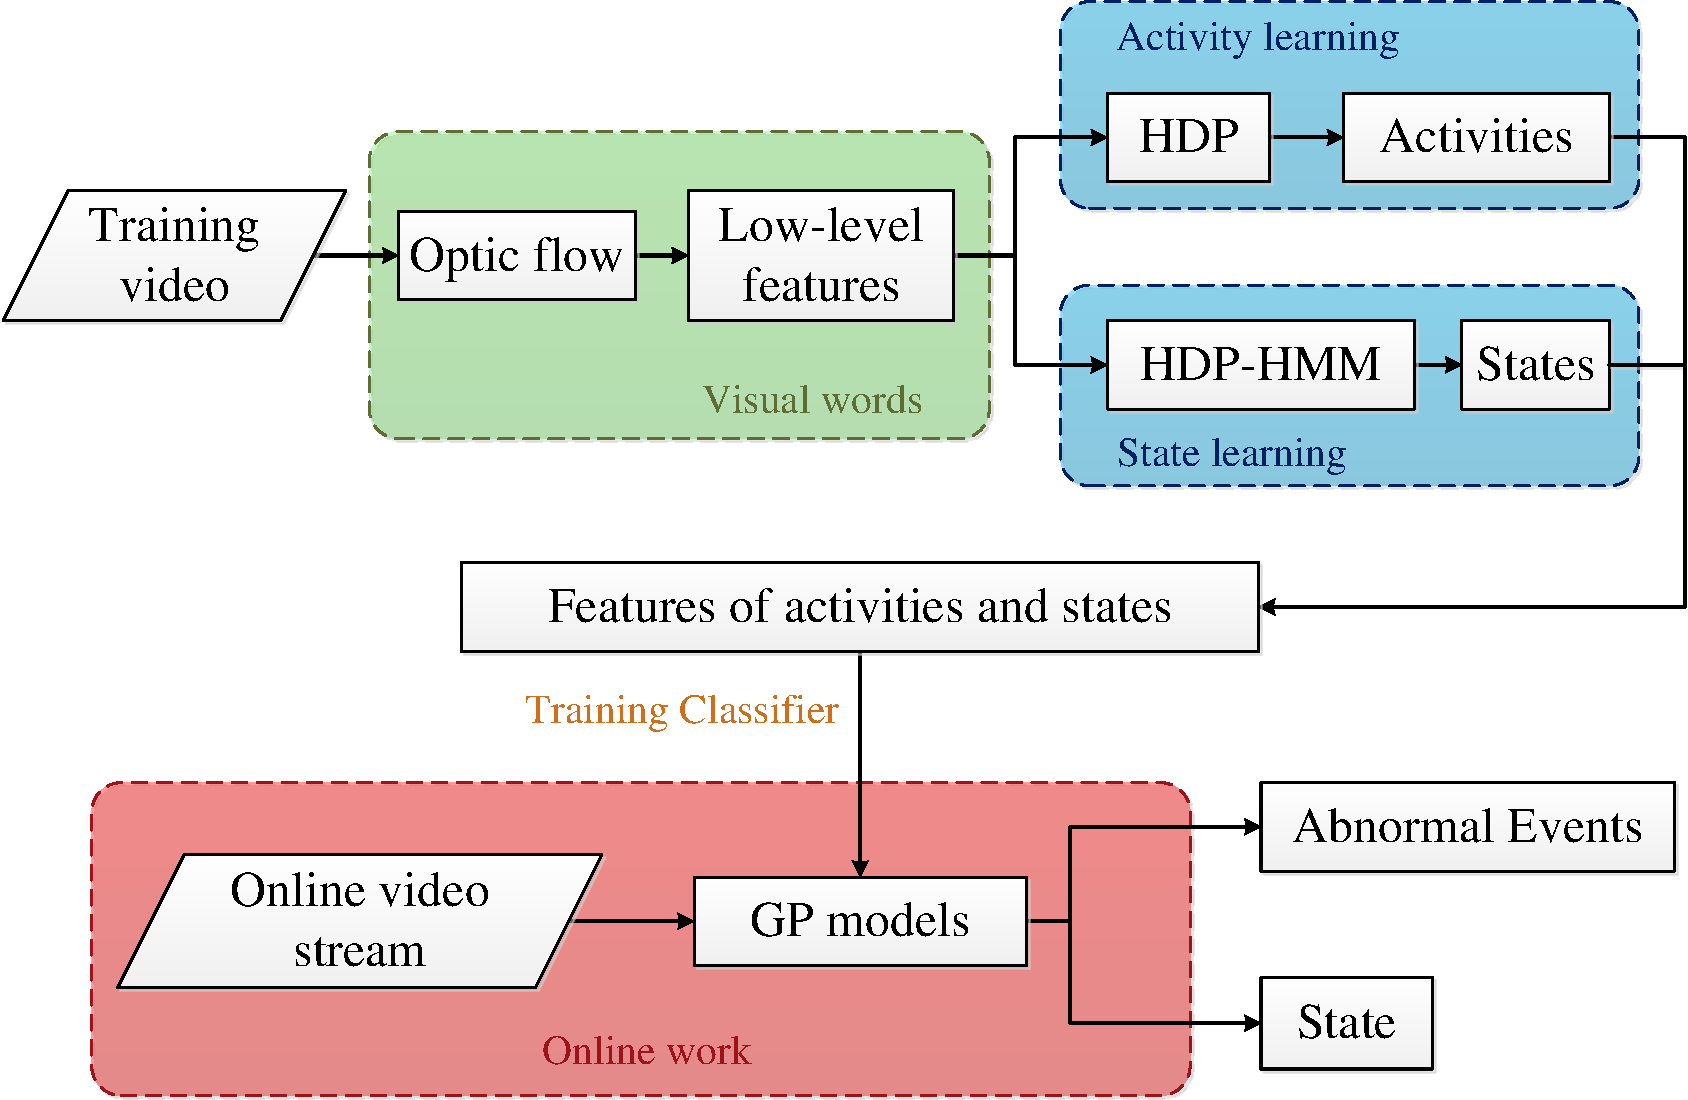
\includegraphics[width = 15cm]{figures/framework-crop.pdf}
	\caption[An overview of our proposed framework]{An overview of our proposed framework}
	\label{fig:framework}
\end{figure}

\section{Low-Level Motion Features}
\label{framework:low-level}
Our datasets are composed of three surveillance video sequences from far-field busy traffic scenes and each is captured by a fixed camera (See Fig.~\ref{fig:traffic_junction}). Since myriads of activities and interactions occur simultaneously among a large number of agents, the general features such as detection and tracking based features are difficult to be extracted in the complicated scenarios. In these situations the local motion features are more reliable and easy to extract. 
%There are a large number of agents of interest. Because of the low resolution, they are small, blurry, crowded and indistinguishable.
%Myriads of activities and interactions occur simultaneously. Many challenging problems are also involved, such as  noise, occlusions, lighting changes and environmental effects. In contrast to many other features such as detection and tracking based features, local motion feature is much more reliable and easy to extract. 
\begin{figure}[!htbp]
	\centering
	\subfigure[QMUL Junction Dataset]{
		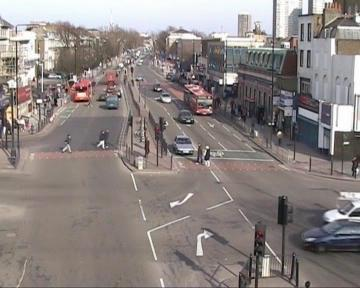
\includegraphics[width = 4.5cm, height=3cm]{figures/qmul.jpg}
	}
	\subfigure[QMUL Junction Dataset 2]{
		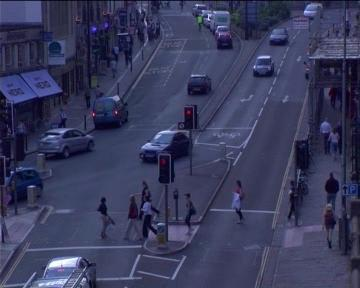
\includegraphics[width = 4.5cm, height=3cm]{figures/qmul2.jpg}
	}
	\subfigure[MIT]{
		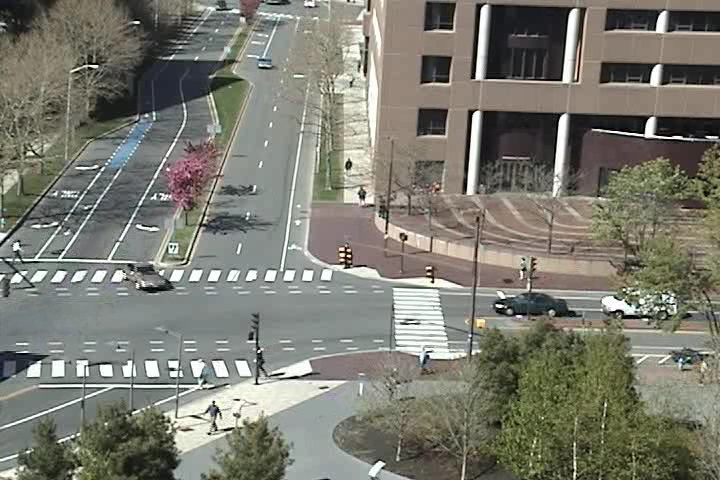
\includegraphics[width = 4.5cm, height=3cm]{figures/mit.jpg}
		\label{fig:mit_exsample}
	}
	\caption[Examples of datasets ]
	{Scenes of three crowded traffic junctions. Each of them is recorded by a fix camera.}
	\label{fig:traffic_junction}
\end{figure}


We represent low-level features using local motions and position features. 
First, we compute optical flow vector for each pixel in each pair of consecutive frames using~\cite{C.Liu_opticflow} (Fig.~\ref{fig:optic_flow}). A proper threshold is necessary to reduce noise: if the  intensity of a flow is greater than the threshold, it is deemed as reliable. 
To obtain rough position features and reduce computation, we spatially divide the camera scene into non-overlapping square cells of size $H\times H$ pixels (Fig.~\ref{fig:pixel_cell}). The selection of $H$ depends on the size of frame.
Each cell local motion feature is the average of all the optical flow vectors within the cell. Then,  each cell local motion feature is quantized into one of the 8 directions (Fig.~\ref{fig:direction}). 
Such discretization necessarily imposes a loss of spatial and directional fidelity. This loss can be reduced by increasing discretization resolution and decreasing $H$ at a cost of increased computation. 
We found it straightforward to set a suitable discretization such that no object was small enough that its motion was missed in the discrete encoding.
Finally, we obtain the low-level visual features in each frame as shown in Fig.~\ref{fig:visual_word}.

\begin{figure}[!htbp]
	\centering
	\subfigure[Pixel cells]{
		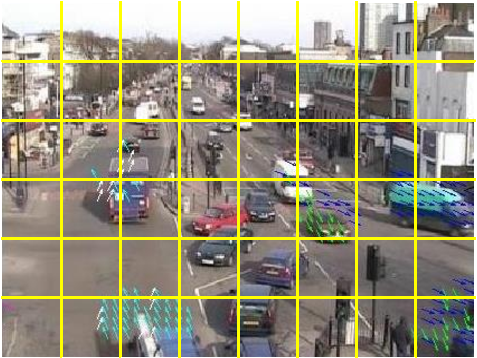
\includegraphics[width = 5.5cm]{figures/pixelcell-crop.pdf} \label{fig:pixel_cell}
	}
	\hspace{1cm}
	\subfigure[Optical flow]{
		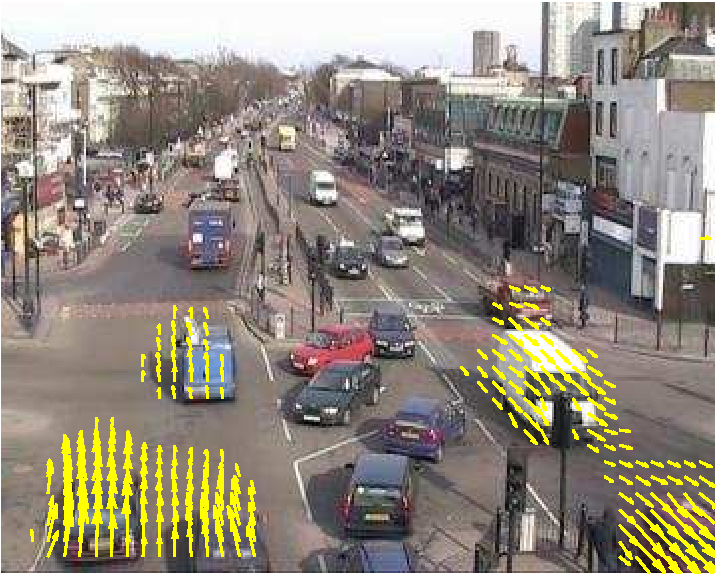
\includegraphics[width = 5.5cm]{figures/of_exsample_3500-crop.pdf} \label{fig:optic_flow}
	}\\
	\subfigure[Quantized direction]{
		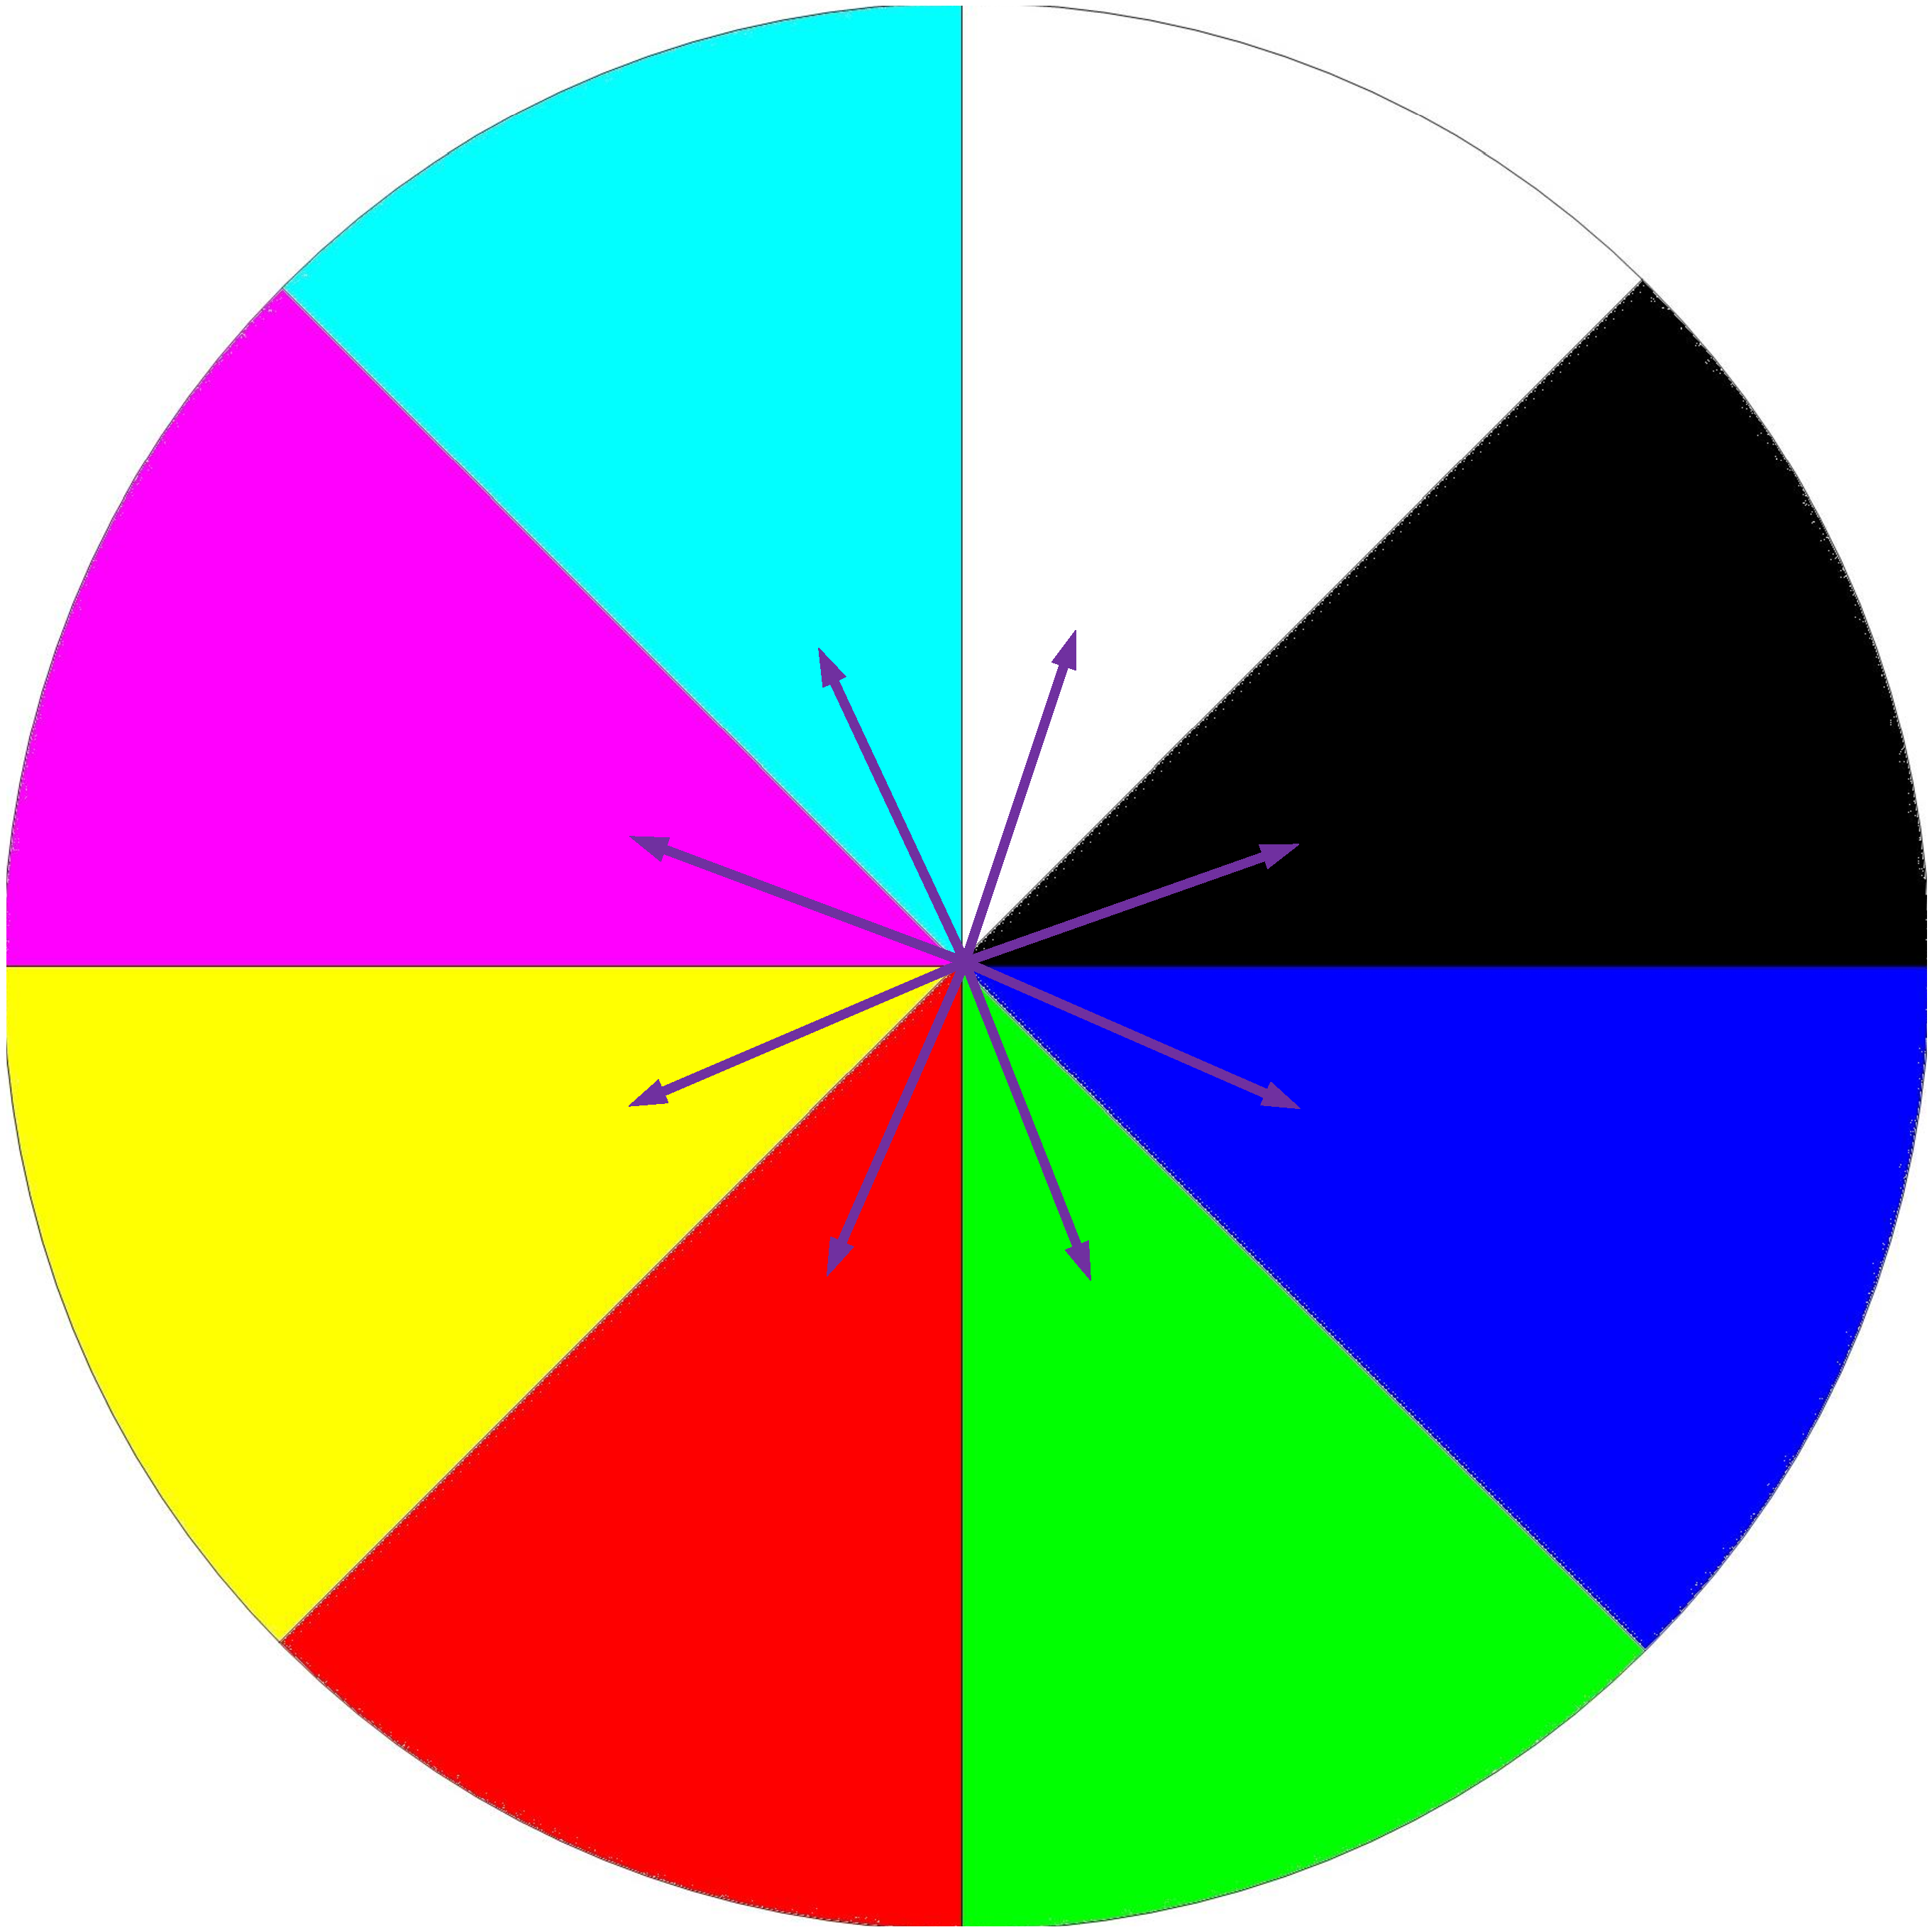
\includegraphics[width = 3.5cm, height=3.5cm]{figures/8directions2-crop.pdf} \label{fig:direction}
	}
	\hspace{3cm}
	\subfigure[Visual words]{
		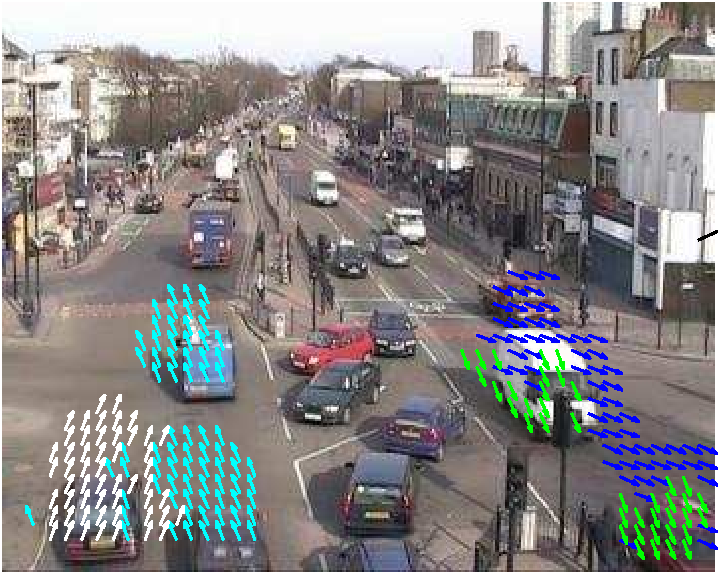
\includegraphics[width = 5.5cm]{figures/word_exsample_3500-crop.pdf} \label{fig:visual_word}
	}
	\caption[low-level visual features extraction]
	{Procedure of low-level visual features extraction.}
	\label{fig:low-level_feature_extraction}
\end{figure}

In this way, a low-level feature is defined as the position of the cell and its motion direction. 
The low-level features are viewed as visual words and they construct a codebook.
For instance, the video dataset from~\cite{wang2009unsupervised} (see Fig.~\ref{fig:mit_exsample}) is $720\times 480$ video frame. If the scene is divide into $10\times10$ square cell, it has a codebook with $72\times48\times8$ visual words. These words may arise in combination in this scene.

An activity is long-term spatial and temporally dynamic object motions, which means that an activity or interaction is abstracted from a video clip instead of between two successive frames.
Therefore, we uniformly segment the input video into non-overlapping clips (see Fig.~\ref{fig:video_clip}). 
Each clip is a collection of local motions occurring in its frames (see Fig.~\ref{fig:words_clip}). 
The local motions that exist in the same clips are viewed as co-occurring. 
Then, the activities are modeled as spatial distribution of local motions.
The problem for representing activities is simplified by ignoring the temporal ordering of local motions within a clip.
In this paper, we empirically select the length of each clip 75 frames, i.e. 3 seconds. If it is too shot, an activity will not completely present and more atomic activities will be clustered. Contrarily, activities may mix with the others and will not be represented precisely.
%In our framework, we treat each video clip as a document, which is a bag of all visual words $\textbf{w}_t$ occurring in clip $t$. The whole input video is a corpus.

\begin{figure}[!htbp]
	\centering
	\subfigure[Video clip]{
		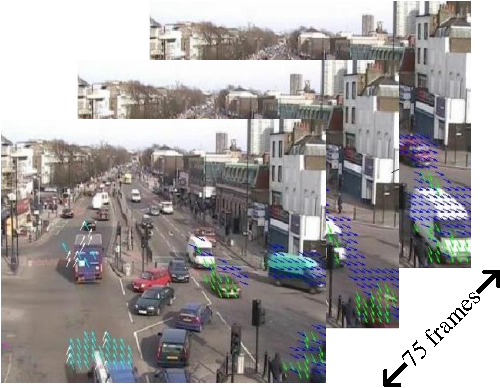
\includegraphics[width = 6.5cm, height=5cm]{figures/clip-crop.pdf}
		\label{fig:video_clip}}
	\hspace{2cm}
	\subfigure[Visual words in a clip]{
		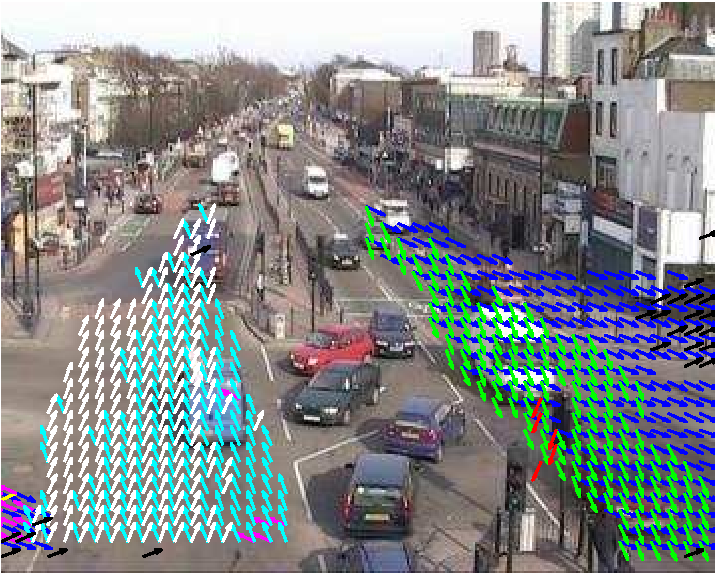
\includegraphics[width = 6cm, height=4cm]{figures/clip_example_clip47-crop.pdf}
		\label{fig:words_clip}
	}
	\caption[Video clip ]
	{(a) A video is uniformly segmented into non-overlapping clips. (b) Each clip is a collection of visual words. }
\end{figure}

All occurring visual words in clip $t$ is noted as a set $\mathbf{x}_t=\{x_{t,i}\}_{i=1}^{N_t}$, where $N_t$ is the total number of occurring motions in clip $t$. We note that the entries in $\mathbf{x}_t$ are unique, which means  we are only interested in the motion occurring during a clip rather than their frequency. One of the most important reasons for using such methods is that, rare motions would not be covered by normal motions. It favors the abnormal events detection. On the other hand, it reduces the quantity of being processed data without loss of useful information.
%This method has two advantages. 
%First, rare motions would not be covered by normal motions. It favors the abnormal events detection. %Second, it is much more easy to represent activities and interactions.
%******************************************************************************

%\section{Model}
%\label{model}
%Our first task is to infer the typical activities and traffic states from video. The low-level features are the exclusive motion information that can be directly observed from the input video. An activity is a mixture of local motions that frequently co-exist in the same clips (or documents). Thus, it is equivalent to infer topics in word-document analysis. Moreover, a traffic state is a combination of frequently co-occurring activities (i.e. interactions). This makes it possible to infer traffic states using topic model, too.  
%
%The HDP~\cite{teh2006hdp} is an unsupervised non-parametric hierarchical Bayesian topic model and was originally proposed for word-document analysis. It clusters the frequently co-occurring words within the same documents into the same topics. Furthermore, different from the other clustering topic models, such as LDA~\cite{blei2003lda}, HDP is able to automatically determine the number of clusters. The rest of this section will show how to use HDP model to infer typical activities and traffic states from the input video. 
%Based on the output of HDP models, we propose a method to construct feature vectors to represent activities with visual words and traffic states with typical activities. Afterwards these will be used to train classifier to online recognize complicated traffic activities in surveillance video.

\section{Learning Activities using HDP}
\label{hdp for activities}
%In this section, we recapitulate HDP to learn activities from video.
% the learning of typical activities from video using HDP models.
The HDP~\cite{teh2006hdp} is an unsupervised non-parametric hierarchical Bayesian topic model which was originally proposed for word-document analysis. It clusters the frequently co-occurring words within the same documents into the same topics. If we treat each low-level feature as a visual word and each video clip as a document of words, activities will be modeled as topics. Therefore, an activity is a multinomial distribution over the visual words and the clip $t$ is explained by the mixture of the activities observed during $t$. 
%For convenient discuss, in the rest of this thesis, we denote $G_0$ as the global list of activities and shared by all clips..

\begin{figure}[t!]
	\center
	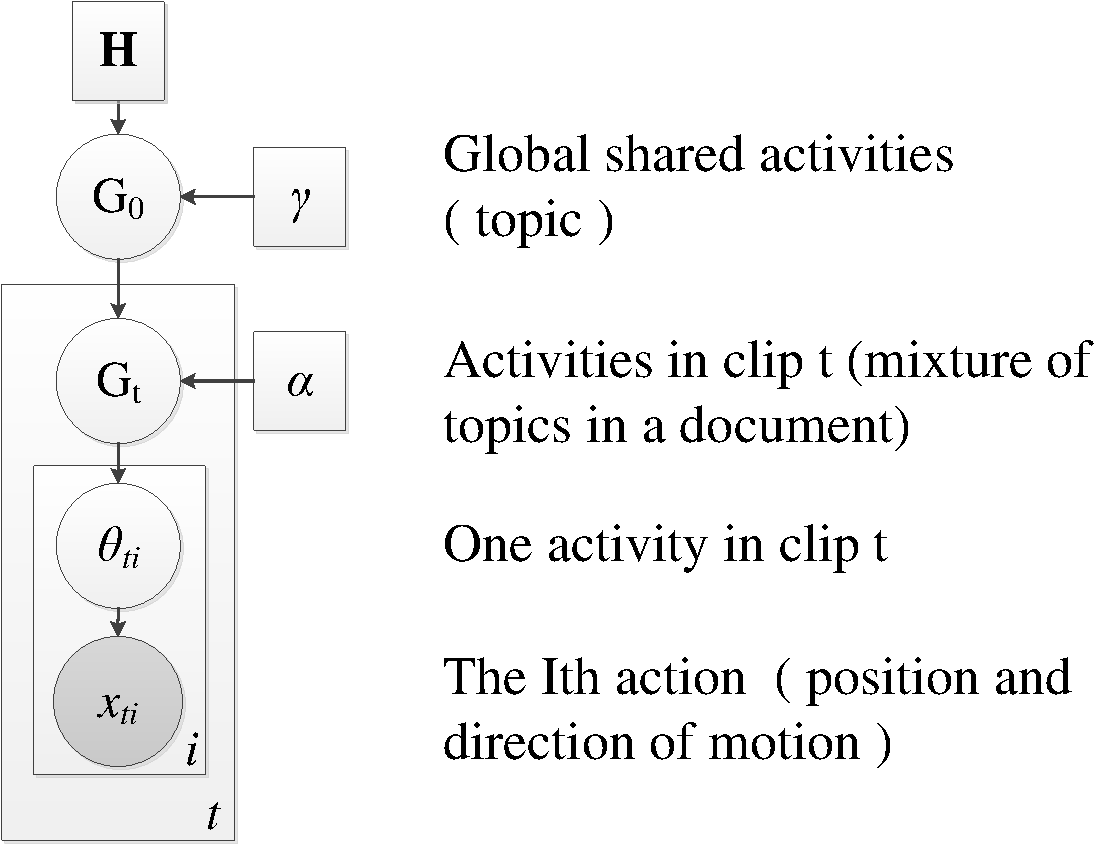
\includegraphics[width=7cm, height =6cm]{figures/HDP_graph-crop.pdf}
	\caption{Activities learning using HDP model}
	\label{hdp_graph}
\end{figure}

The activities are learned using the standard HDP model as shown in Fig.~\ref{hdp_graph}. To be suitable in our case, the meaning of each element in the graph is redefined as the annotation. The global random measure $G_0$ is the global activities (topics) set shared by all clips. Its distribution is a Dirichlet Process with concentration parameter $\lambda$ and Dirichlet prior $H$:
\begin{equation*}
	G_0|\gamma,H \thicksim DP(\gamma,H),
\end{equation*}
$G_0$ can be expressed using the stick-breaking formulation~\cite{teh2006hdp}:
\begin{align*}
	G_0 = \sum^\infty_{k=1}\pi _k\delta_{\phi_k},&~~\pi_k =\pi _k'\prod^{k-1}_{l=1}(1-\pi _l'),\\
	\pi_k'\thicksim Beta(1,\lambda),&~~\phi_k|\gamma,H \thicksim H,
\end{align*}
where $\{\phi_k\}$ is parameter set of multinomial distributions over words in codebook corresponding to topic $\theta_k$, i.e. word probability vector. It is is generated from $H$. $\delta_{\phi_k}$ is the Delta function at point $\phi_k$. $\{\pi_k\}$ are random probability measures (mixtures over activities).
%and $\Sigma_{k=1}^\infty \pi_k=1$. It is also known as $\pi_k \thicksim GEM(\gamma)$ in stick-breaking process. 
%It can be interpreted as mixtures over topics.
%The multinomial distribution $\phi_k$ over words in the codebook is generated from $H$. 
%Therefore, $H$ is interpreted as a distribution over multinomial distributions and defined as a Dirichlet distribution:
%\begin{align*}
%H = Dir(D_0),~~\phi_k|\gamma,H  \thicksim Dir(D_0).
%\end{align*}

$G_t$ is a random measure and drawn from the second DP with concentration parameter $\alpha$ and Dirichlet prior $G_0$:
\begin{equation*}
	G_t|\alpha,G_0 \thicksim DP(\alpha,G_0),
\end{equation*}
where $G_0$ itself is drawn from the first DP as demonstrated above. Thus, $G_0$ is a prior distribution over the whole corpus and a sample $G_t$ is a subset drawn from $G_0$. In our case $G_t$ describes the multinomial distribution of active topics in clip $t$, i.e. activity probability vector for clip $t$. We express it using the stick-breaking representation again as
\begin{align*}
	G_t = \sum^\infty_{k=1}\pi _{tk}\delta_{\phi_k},&~~\pi_{tk} =\pi _{tk}'\prod^{k-1}_{l=1}(1-\pi _{tl}'),\\
	\pi_{tk}'\thicksim Beta(1,\alpha),&~~\phi_k|\alpha,G_0 \thicksim G_0.
\end{align*}
For the $i$th word in document $t$, a topic $\theta_{ti}$ is first drawn from $G_t$ and then the word $x_{ti}$ is drawn from multinomial distribution $Multi(x_{ti};\phi_{\theta_{ti}})$. 
%Notice that, different $G_t$ has the same ${\phi_k}$ as $G_0$, which means different clips share the same set of topics and statistical strength. 
We use Gibbs sampling schemes to do inference under an HDP model, which is adopted in~\cite{teh2006hdp}. %Fig.~\ref{qmul_activity} shows the learned typical activities by HDP models for QMUL Junction Dataset~\cite{hospedales2009markov}.

The hyper-parameters $\gamma$ and $\alpha$ are priors on the concentration of the word distribution within activities. They affect the the number of activities in $G_0$ and $G_t$. Furthermore, $D_0$ is the parameter for the Dirichlet distribution $H = Dir(D_0)$. In general, higher elements in $D_0$ produce less variance in samples from $H$. We will discuss how to select these hyper-parameters in Sec.~\ref{parameter}.

Although HDP models decide the number of topics automatically, some of the mined activities have no meaning.
They could be induced by noise or rare events (see Fig.~). 
Their existence might lead to ambiguous or even misleading analysis of interactions.
Therefore, we need to select the typical activities which are representative in this scene. Based on the learning results from HDP, we first compute the ratio of each activity occurring in given video. Throughout the video clips, the amount of words that are assigned with label of activity $k$ is noticed as $n_k$. The occurrence ratio of activity $k$ within all the clips is
\begin{equation}
	r_k = \frac{n_k}{n_1+\cdots+n_K}. 
\end{equation} 
We rank $\{r_1,\cdots,r_K\}$ in decreasing order as $\mathbf{r'}=\{r'_1\geq \cdots \geq r'_K \}$ and calculate the accumulated sum of $\mathbf{r'}$
\begin{equation}
	R'_j = \sum_{i=1}^{j} r'_i. 
	\label{eq:accusum} 
\end{equation} 
The typical activities set is determined as
\begin{equation}
	\mathbf{A_{typical}}\triangleq\{A_j|R'_j \leq 0.99\},~~1\leq j \leq K,
	\label{eq:Atypical} 
\end{equation} 
where $A_j$ denotes activity $j$ with ratio $r'_j$. 
We execute this process for two reasons. First,to represent a normal interaction only the typical activities are meaningful. Deletion of rare occurring activities makes the system more sensitive to abnormal events. Second, reduction the number of activities also means the reductions of features of high-level events in our case. In Chap.~\ref{chap:experiment} we will illustrate it in detail.
%-----------------------------------------------------------------------


\section{Learning States Using HDP-HMM}
\label{framework:hdp-hmm}
In this thesis, one of our goals aims at recognizing the traffic states during each clip, which is in our case regarded as a high-level event.
Therefore, the typical traffic states need to be learned in the given scene primarily.
%We model a traffic state as a combination of activities. 
Similar to learning activities from visual words, HDP models are also applicable to cluster video clips into some states based on the co-occurring words during the same clips.
%a HDP model is also applicable to cluster frequently co-occurring activities (interactions) during the same clips into the same traffic states, i.e. clustering clips. 
In addition we notice that, a traffic scene is regulated by traffic lights, i.e., the transition rule of traffic states is circulatory. Therefore, a Hidden Markov Model (HMM) is worth to be considered here.

\begin{figure}[!htbp]
	\center
	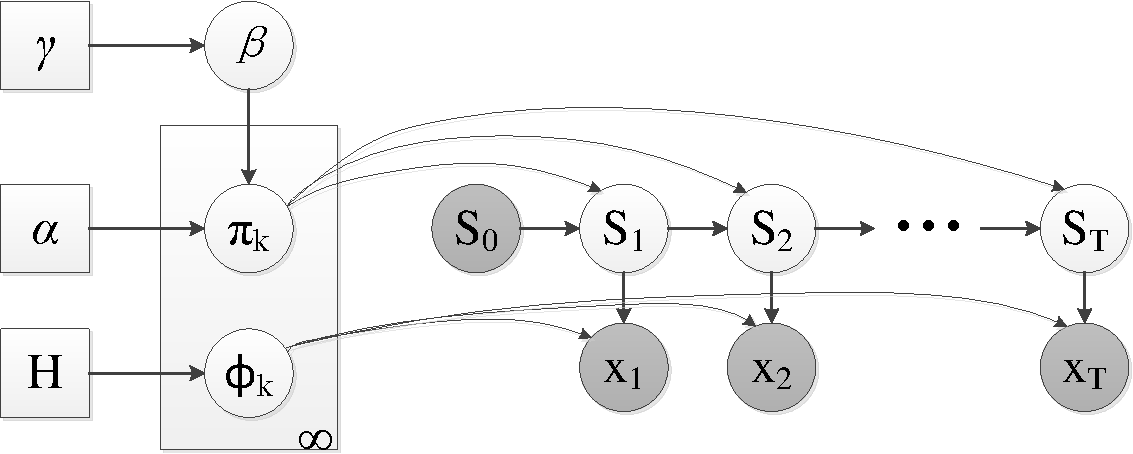
\includegraphics[width=8.5cm, height =4cm]{figures/HDP-HMM-crop.pdf}
	\caption{A graphical representation of the HDP-HMM model}
	\label{hdp_hmm}
\end{figure}

HMM can be explained as a doubly stochastic Markov chain and is essentially a dynamic variant of a finite mixture model. By replacing the finite mixture with a Dirichlet process, a HDP-HMM model illustrated as~Fig.~\ref{hdp_hmm} was proposed in~\cite{teh2006hdp}. Its stick-breaking formalism is:
\begin{align*}
	& \beta \thicksim GEM(\gamma), ~~\mathbf{\pi}_k \thicksim DP(\alpha,\beta),~~ \phi_k \thicksim H ,\\
	& s_t|s_{t-1} \thicksim Mult(\mathbf{\pi}_{s_{t-1}}),~~\mathbf{x}_t|s_t \thicksim Multi(\phi_{s_t}),
\end{align*}
where $s_t$ is the state of clip $t$ and $\mathbf{x}_t$ is its observation set. In this case, each vector $\mathbf{\pi}_k=\{\pi_{kl}\}_{l=1\cdots L}$ is one row of the Markov chain's transition matrix from state $k$ to other states and $L$ is the total number of states. For a better illustration, we denote these transition matrix as $\mathbf{M} = \{m_{i,j}\}_{i,j=1\cdots L}$ throughout this paper.
In this model, our target is decoding the $s_t$ hidden variables which correspond to the state classes. 
%The latent variables $\pi_t$, we also adopt Gibbs sampling schemes to do inference under this HDP-HMM.
%Fig.~\ref{qmul_state} shows the typical traffic states learned by HDP-HMM model for QMUL Junction Dataset~\cite{hospedales2009markov}.

Same as the learning of activities with HDP models, traffic states mined by HDP-HMM models are more than necessary. The typical traffic states are also selected in the similar way. We denote $n_i$ as the number of clips which are assigned with state $i$. Its ratio in all clips is defined as:
\begin{equation}
	r_s = \frac{n_i}{n_1+\cdots+n_S},
\end{equation} 
where $S$ is the total number of states learned by HDP-HMM models. The following two steps are same as Eq.~\eqref{eq:accusum} and~\eqref{eq:Atypical}. The set of typical states is
\begin{equation}
	\mathbf{S}_{typical} \triangleq \{s_j|R'_j \leq 0.9\},~~1\leq j \leq S.
\end{equation} 
In Chap.~\ref{chap:experiment} we will illustrate it in detail.
%------------------------------------------------------------------------

\section{Representation of Activities and States}
\label{framework:representation}

Traditional approaches represent each video clip as a set of low-level features and encode it into a fixed length feature vector, e.g. Bag-of-words. 
However, there is a big gap between low-level features and high-level events. 
Therefore, based on the learning results of activities and states, we introduce a method to represent activities using low-level visuals features and states using typical activities. 

\subsection*{Representation of Activities}
In the HDP models, activities are modeled as multinomial distribution over words in codebook. However, these probabilities are not suitable to be directly used as features by classifier. 
Hu et al.~\cite{hu2009abnormal} proposed a method based on Fisher kernel using the learned probability distribution in a one-class SVM classifier. 
Their method requires gradient of the log likelihood with respect to parameter of the model. 
However, the number of the parameters of the model is usually large. In our case, it equals the total number of activities which is larger than 20 (See Chap.~\ref{chap:experiment}). 
Hence, the partial differential is really complex in mathematics and computations consuming. 
Furthermore, before classifying they must first compute the joint distribution using iterative sweeps of Gibbs sampler.
\begin{figure}[!htbp]
	\centering
	\subfigure[All possible visual words (left) and their distribution]{		
		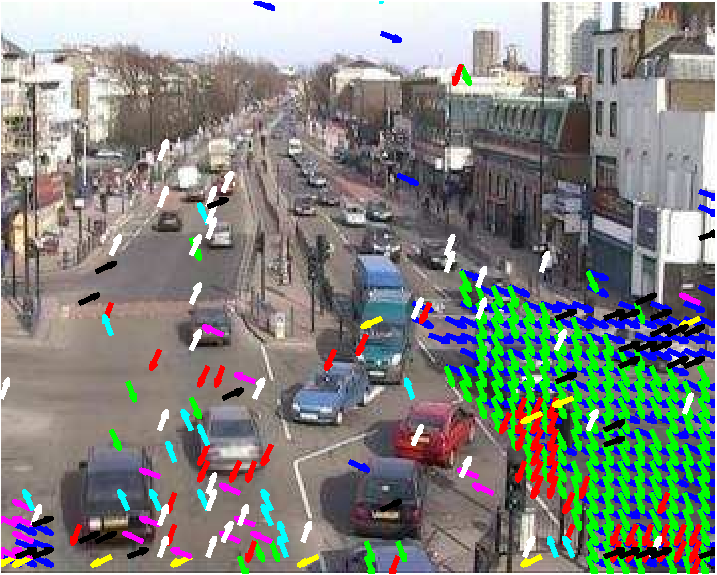
\includegraphics[width=5cm, height=4cm]{figures/topic1_orig-crop.pdf}
		\hspace{1cm}
		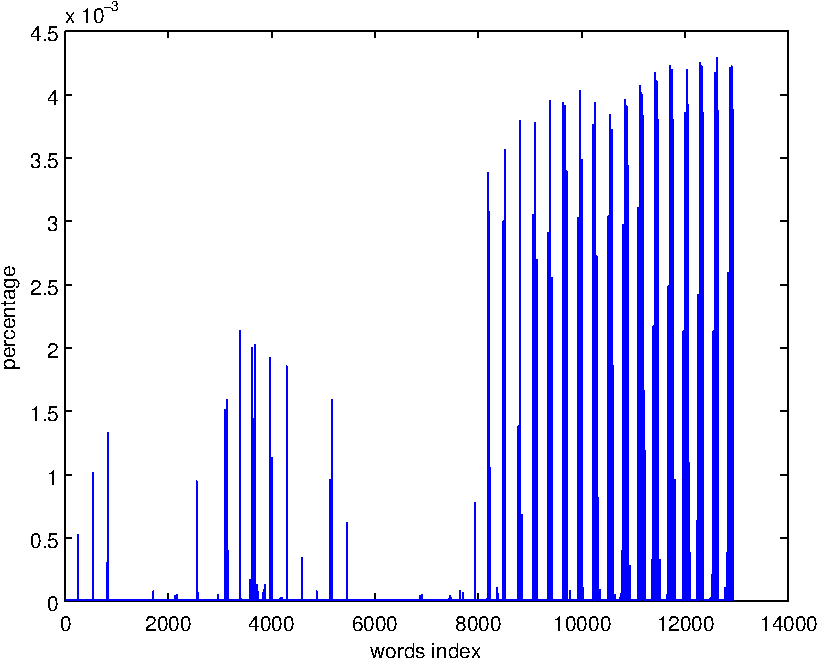
\includegraphics[width=7cm, height=4.5cm]{figures/topic1_words_distribution_org-crop.pdf}
		\label{fig:subfig:all_words}
	}\\
	%\hspace{2cm}
	\subfigure[Dominant visual words (left) and their distribution]{
		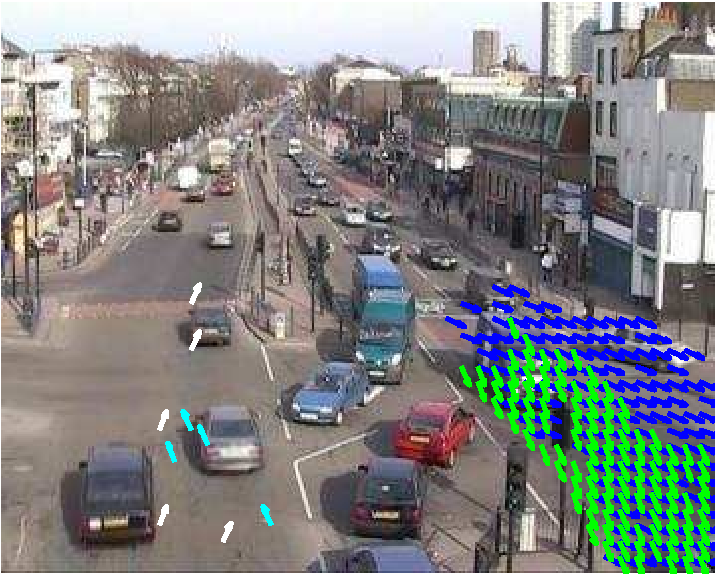
\includegraphics[width=5cm, height=4cm]{figures/topic1_pattern-crop.pdf}
		\hspace{1cm}
		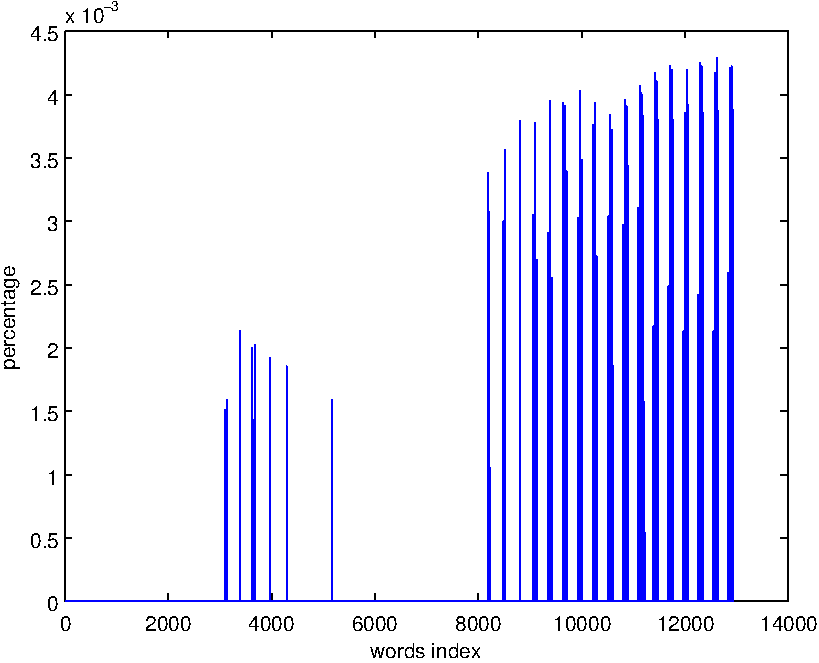
\includegraphics[width=7cm, height=4.5cm]{figures/topic1_words_distribution_dominant-crop.pdf}
		\label{fig:subfig:dominant__words}
	}
	\caption[Activity patterns]
	{An example of activity pattern. (a) All possible words that have larger than 0 probability to occur in this activity. The probability of each word is shown in the right histogram.(b) The dominant words that are determined by Eq.~\eqref{0.9 words in topic}. The distribution of remaining words is shown in the right histogram.}
	\label{Activity patterns}
\end{figure}

To address this problem, we extract the dominant visual words to construct activity patterns based on the multinomial distribution over words of a activity.
Each activity $k$ has an corresponding multinomial distribution $\phi_k$ over the words in codebook noticed as $\phi_k = \{\phi_{kw_i}\}_{i=1}^{N_w}$, where $\Sigma_{i=1}^{N_w} \phi_{kw_i}=1$
%$\mathbf{p}_{k\mathbf{w}} = \{p_{kw_i}\}_{i=1}^{N_w}$, $\Sigma_{i=1}^{N_w} p_{kw_i}=1$
and $N_w$ is the size of codebook.
The entries of $\phi_k$ are sorted in descending order according to their probabilities $\mathbf{p}_{k\mathbf{w}} = \{p_{kw_1}\geq\cdots\geq p_{kw_{N_w}}\}$. Then we calculate the accumulated sum of probability as

\begin{equation}
	p'_{kj} = \sum_{i=1}^{j<N_w} p_{kw_i}.
	\label{aaccumulated_sum}
\end{equation}
%the subscript ''as'' means ''accumulated sum'' for convenience.
The dominant visual words for topic $k$ are denoted as:

\begin{equation}
	\mathbf{w}_k= \{w_j|p'_{kj}\leq 0.9 \},~~1\leq j<N_w .
	\label{0.9 words in topic}
\end{equation}

The word set $\mathbf{w}_k$ can be explained as the most frequently co-occurring motions in activity $k$. 
The rest of the words which fall into the rest $10\%$ are viewed as rare occurring motions. They could be caused by noise or abnormal events. 
The pattern of activity $k$ is then represented using the word set $\mathbf{w}_k$. 
An example for the activity of vehicles driving downward is shown in~Fig.~\ref{Activity patterns}.
Fig.~\ref{fig:subfig:all_words} shows the spatial distribution of all possible co-occurring visual words for this activity. The most frequently occurring words determined by~Eq.~\eqref{0.9 words in topic} are shown in~Fig.~\ref{fig:subfig:dominant__words}.
In contrast to Fig.~\ref{fig:subfig:all_words}, Fig.~\ref{fig:subfig:dominant__words} eliminates most of ambiguous and rambling visual words. 
%Our method is effective to reduce the influence caused by noise or anomaly.

%Our representation has following advantages: 1) we are only interested in the. 2) rare motions are easy detected without complex computation.

\subsection*{Representation of Global Interactions} 
Activity patterns from the aforementioned step are varying in length. They are not suitable to directly represent the global interactions in a clip. 
Therefore, we introduce a method to encode activities to characterize interactions.
$\mathbf{x}_t=\{x_{ti}\}_{i=1}^{N_t}$ is the set of visual words in clip $t$, and $N_t$ denotes the amount of words. We compare each activity pattern $\mathbf{w}_k$ with $\mathbf{x}_t$ and calculate the percentage of the intersection as
\begin{equation}
	p_{tk} = \frac{\mathbf{x}_t \cap\mathbf{w}_k}{N_t}.
	\label{eq:clip_feature}
\end{equation}
It explains the ratio of motions $\mathbf{x}_t$ which can be explained by activity $k$ in this clip. Then, the feature vector of clip $t$ consists of $\mathbf{c}_t=\{p_{t1},\cdots,p_{tK}\}$. Such features can be explained as the components of an interaction. We note that the sum of $\mathbf{c}_t$ is not guaranteed to equal one, because some visual words may belong to some activities simultaneously, or some rare motions do not belong to any activities. Therefore, it needs to be normalized.
For more intuition, we will illustrate it in Chap.~\ref{chap:experiment} with specific examples.


\section{Online GP Classification}
\label{framework:gpc}

All of the video clips for training have been clustered by HDP-HMM model and their label set is $\mathbf{y}=\{y_1,\cdots,y_T\}$, where $T$ is the total number of clips. $\mathbf{c}_t$ is the feature vector of clip $t$ given by Eq.~\eqref{eq:clip_feature}, and $\mathbf{C}=\{\mathbf{c}_1,\cdots,\mathbf{c}_T\}$. Then, the training dataset is $(\mathbf{C},\mathbf{y})$ and used to train the supervised classifier. We apply one-against-all strategy for multiclass classifying task in this thesis due to its probabilistic output which will be useful in later procedure. 
Therefore, for each class of traffic states a classifier is necessary to be trained with the samples of the corresponding class as positive samples $y=+1$ and all other samples as negatives $y=-1$.

To classify traffic states in an online captured video sequence, each new coming 75 frames from video stream are segmented into a clip. Hence, our task is labeling the new coming video clip $\mathbf{c}^*$ to a traffic state which has the highest probability $p(y^*|\mathbf{C},\mathbf{y},\mathbf{c}^*)$. 
As we have discussed in Sec.~\ref{framework:gpc}, in a classifier for class $s_j$ the probabilistic prediction for test clip $c^*$ is assigned with label $y^*=+1$ as:
\begin{equation}
	p(y^*=+1|\mathbf{C},\mathbf{y},\mathbf{c}^*)|_{y^*=s_j} = \int p(y^*|f^*)p(f^*|\mathbf{C},\mathbf{y},\mathbf{c}^*) df^*. \label{GPCprob}
\end{equation}
Then the traffic state of clip $\mathbf{c}^*$ is
\begin{equation}
	y^* = \arg\max_{s_j}~p(y^*=+1|\mathbf{C},\mathbf{y},\mathbf{c}^*)|_{y^*=s_j}.
	\label{gp_label}
\end{equation}




\section{Integration of Transition Information into GP Classifier}
\label{framework:gp+hmm}
The input video is segmented into clips along time. 
It cannot be ensured that each clip precisely involves only a traffic state. 
In practice, sometimes the transition between two states occurs in a clip. 
For example as shown in~Fig.~\ref{fig:ambiguous_state}, the state is ambiguous and hard to decide whether it is a leftward or rightward flow.
Sometimes the scene is silent in some clips: there are very few or no motions, as shown~Fig.~\ref{fig:silent_scene}. 
In this case, the GP classifier will label it with the state which has highest probabilistic prediction as Eq.~\eqref{gp_label}. 
Furthermore, sometimes a complete behavior is divided into two activities due to the video clip segmentation as shown in Fig.~\ref{fig:bad_segmentation}. The vehicles from bottom are turning right and driving out the camera scene. However, the tail of this behavior presents as a rightward flow (see the right figure). GP classifier may classify it as the traffic state of rightward flow.
Fortunately, a crowded traffic scene is normally regulated by traffic lights. 
The transition between two traffic states is rule-based, e.g., the transition from state~Fig.~\ref{fig:subfigure:state1} to state~Fig.~\ref{fig:subfigure:state3} is forbidden.
%With the help of transition Information, the classification results could be enhanced.
\begin{figure}[!htbp]
	\centering
	\subfigure[Silent scene]{
		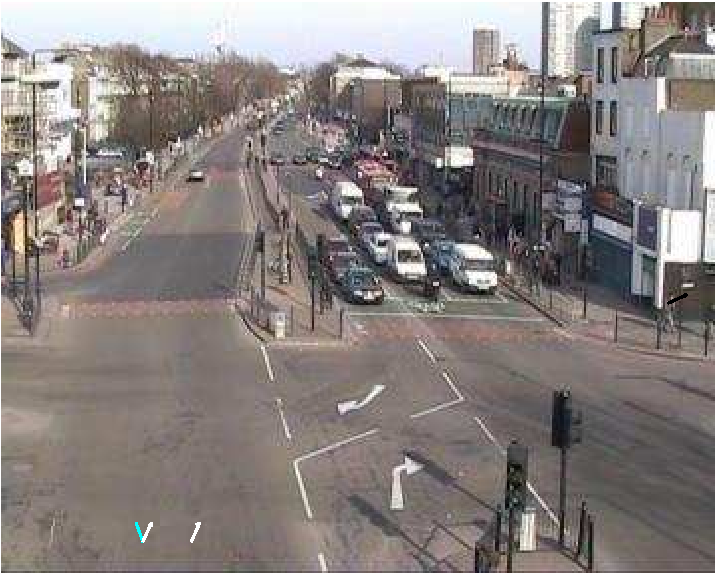
\includegraphics[width = 5cm]{figures/silence_exsample-crop.pdf}
		\label{fig:silent_scene}
	}
	\hspace{1cm}
	\subfigure[Ambiguous state]{
		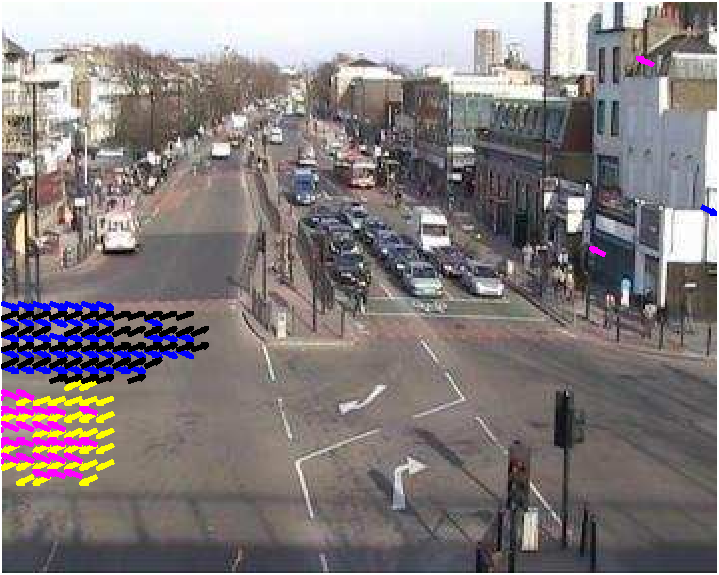
\includegraphics[width=5cm]{figures/qmul_topic/false_sample1-crop.pdf}
		\label{fig:ambiguous_state}
	}
	\subfigure[A complete behavior is divided into two different ones due to video clip segmentation]{
		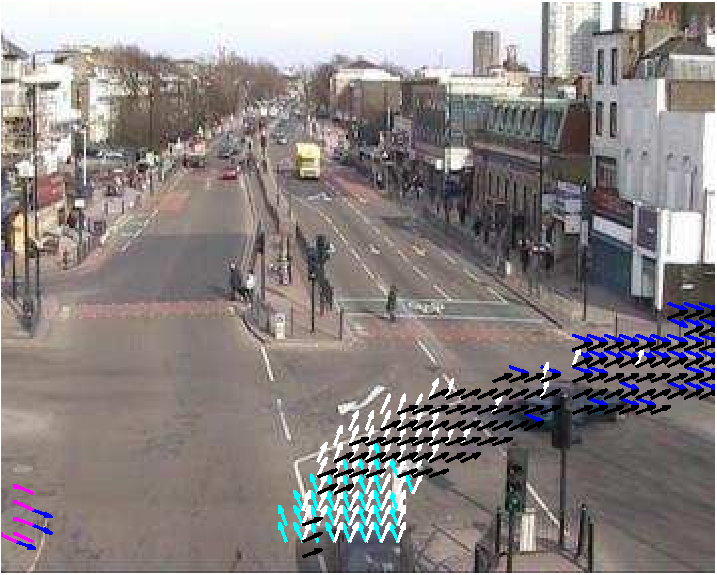
\includegraphics[width = 5cm]{figures/transistion_exsample1-crop.pdf}
		\hspace{1.3cm}
		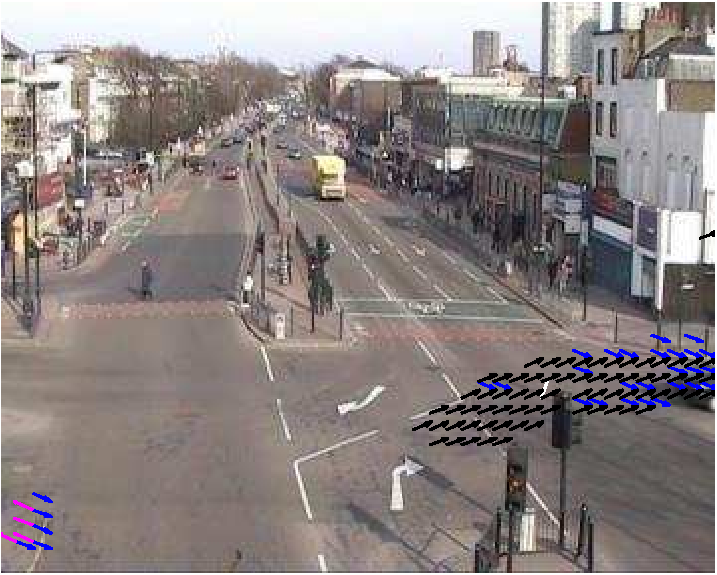
\includegraphics[width = 5cm]{figures/transistion_exsample2-crop.pdf}
		\label{fig:bad_segmentation}
	}
	\caption[Examples of hard being exactly recognized scenes by GP classifier.]
	{Examples of possible challenges for GP classifier to exactly classify the traffic state.}
	\label{fig:transition_exsample}
\end{figure}
The classification result given by the GP classifier could be corrected with the assistance of the temporal dependencies between two states. 
For this purpose, a state energy is defined for clip $t$ being assigned as state label $y_t=s_i$ as follows:
\begin{align}
	E(y_t=s_i|y_{t-1}=s_j) &= -log\{p(y_t=s_i|\mathbf{c}_t)\}-\beta~log~(p(s_i|s_j)) (1-\delta(s_i,s_j)),\\\label{eq:gphmm}
	y_t &= \arg\min_{s_i}E(y_t=s_i|y_{t-1}=s_j),
\end{align}
where $p(y_t=s_i|\mathbf{c}_t)$ is the likelihood of clip $t$ labeled as state $s_i$ given by Eq.~\eqref{GPCprob}. $p(s_i|s_j) = m_{s_i,s_j}$ is the transition probability from state $s_j$ (state of previous clip) to $s_i$ which has been given in Sec.~\ref{framework:hdp-hmm}. $\beta$ is the weight coefficient of transition energy and is set experimentally. $\delta(s_i,s_j)=1,~\mbox{if}~i=j,~\mbox{otherwise}~0$. 
It means that, if the state does not change compared with previous clip, the temporal dependencies is not necessary to be considered. If the state changes, the transition information is taken into account to enhance the classification accuracy. The state which has minimal state energy is selected. 
However, the transition between two states really rarely or never happen, which means that $m_{s_i,s_j}\approx 0$ and leads to an infinity $log(p(s_i|s_j))$ in Eq.~\eqref{eq:gphmm}. It may lead to a completely wrong result.
%It will destroy the balance between classification and transition information. 
To prevent this case, a limitation is necessary for Eq.~\eqref{eq:gphmm} defined as:
\begin{equation}
	p(s_i|s_j)=
	\begin{cases}
		m_{s_i,s_j},  & \mbox{if~} m_{s_i,s_j}\geq Th_{state}\\
		1, & \mbox{otherwise}
	\end{cases}
\end{equation}
where $Th_{state}$ is the threshold for transition probability and set it as $0.1$ in this thesis.
It means that, if a rare or impossible state transition occurs, the recognition results will be completely determined by the GP classifier. This processing mode benefits the abnormal events detection as discussed in Sec.~\ref{framework:abnormal}.

Notice that, if the scene is silent, we prefer to remain the same state as previous clip to reduce confusion. Then a limitation for GP classifier is defined as: 
%We define a limitation for GP classifier in the silent scene as 
\begin{equation}
	p(y_t=s_j|\mathbf{c}_t)=
	\begin{cases}
		p(y^*=+1|\mathbf{C},\mathbf{y},\mathbf{c}^*)|_{y^*=s_j},  & \mbox{if~} N_t\geq Th_{word}\\
		1, & \mbox{otherwise}
	\end{cases}
\end{equation}
where $Th_{word}$ is the threshold of the total number of visual words in a clip. If it is too small, the noise words would deeply affect the judgment. In contrast, the subtle abnormal motions would not catch attention. Considering such busy scene with crowded motions, each of which is represented by a visual word of a $8\times 8$ pixel block, we set it as $30$ empirically. In a silent scene $p(y_t=s_i|\mathbf{c}_t)=1$ means that this clip could be in any typical state. Then, $y_t$ has the same label as its previous clip.


\section{Abnormal Events Detection}
\label{framework:abnormal}
Abnormal events identification is always one of the most interesting and desired capabilities for automated video behavior analysis. 
However, dangerous or illegal activities often have few or possible only one prior example to learn from and are often subtle. 
In other words, it is a challenging problem for identifying abnormal events according to their motion patterns for supervised classifier. 
To tackle this problem, the abnormal events should be defined at first. They are roughly categorized into three groups.

\begin{figure}[!htbp]
	\centering
	\subfigure[Ambulance diving in lane]{
		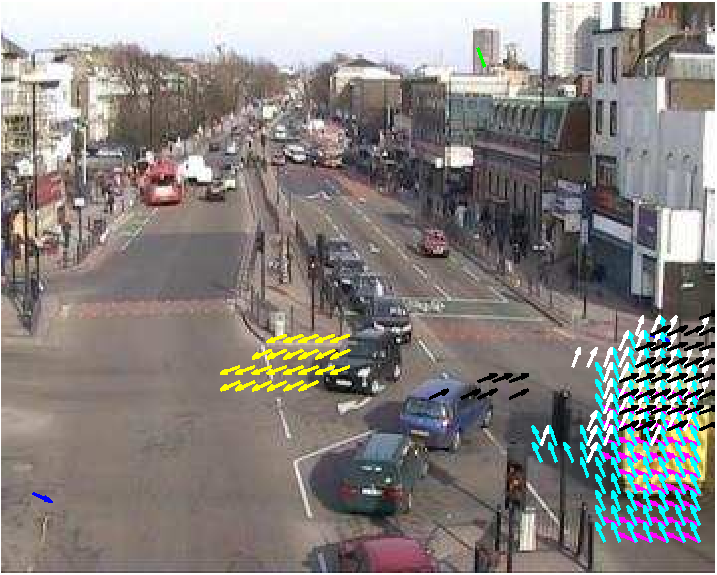
\includegraphics[width=5cm]{figures/qmul/ambulance_212-crop.pdf}
		\label{fig:ambulance_exsample}
	}
	\hspace{1cm}
	\subfigure[Police vehicle diving conversely]{
		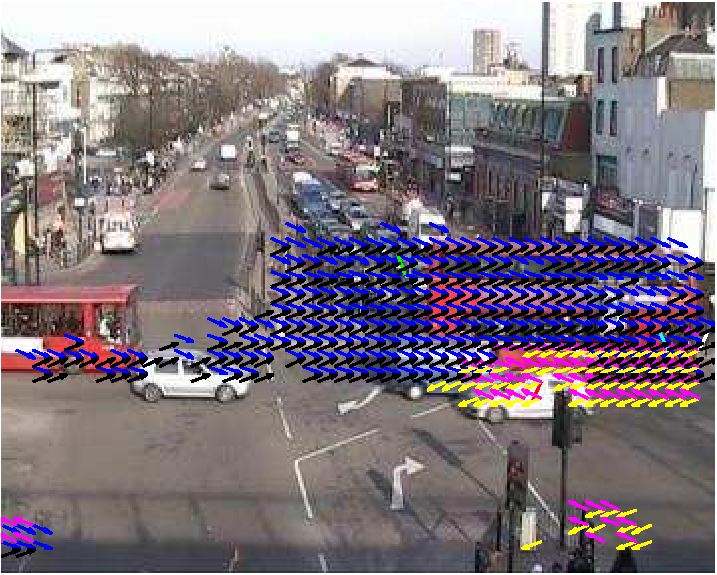
\includegraphics[width=5cm]{figures/qmul/police_892-crop.pdf}
		\label{fig:police_exsample}
	}\\
	
	\subfigure[Traffic state changes due to the fire engine]{
		\begin{minipage}{0.26\textwidth}
			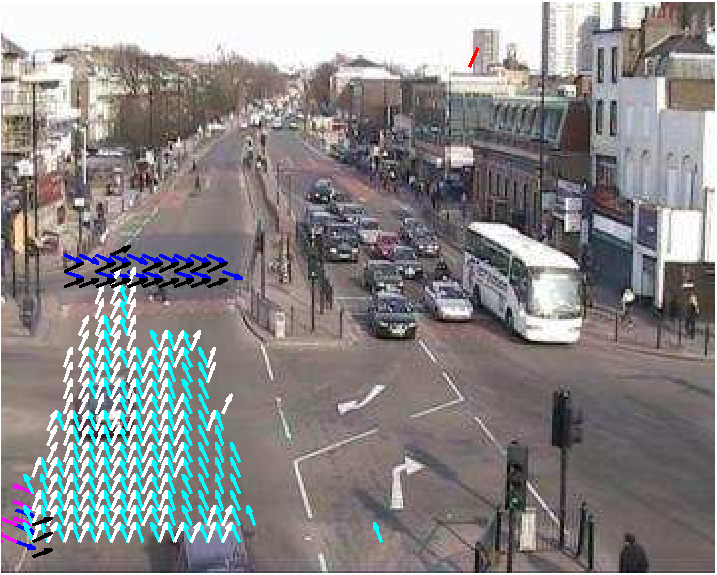
\includegraphics[width=5cm]{figures/qmul/fireengine_412-crop.pdf}\\
			\centering\scriptsize{Vertical flow in $t-1$ clip}
		\end{minipage}
		\hspace{1cm}
		%\caption{Vertical flow in $t-1$ clip}
		\begin{minipage}{0.26\textwidth}
			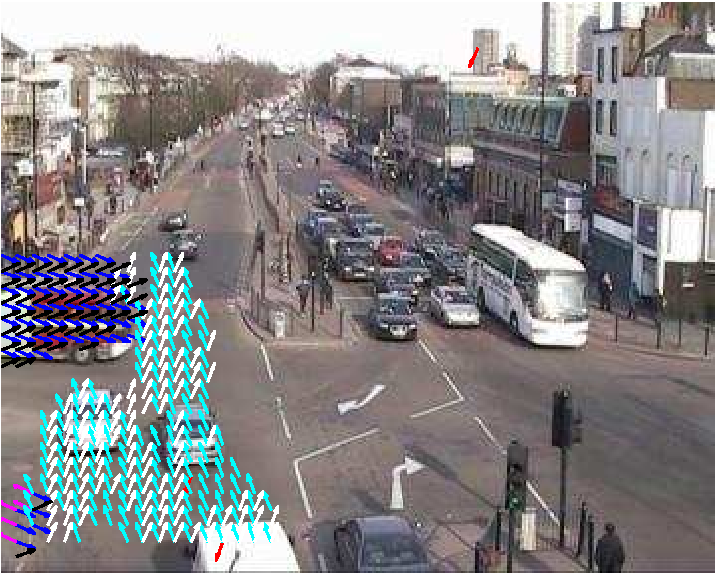
\includegraphics[width=5cm]{figures/qmul/fireengine_413-crop.pdf}
			\centering\scriptsize{Fire engine presents in $t$ clip}
		\end{minipage}
		\hspace{1cm}
		%\caption{Fire engine present in $t$ clip}
		\begin{minipage}{0.26\textwidth}
			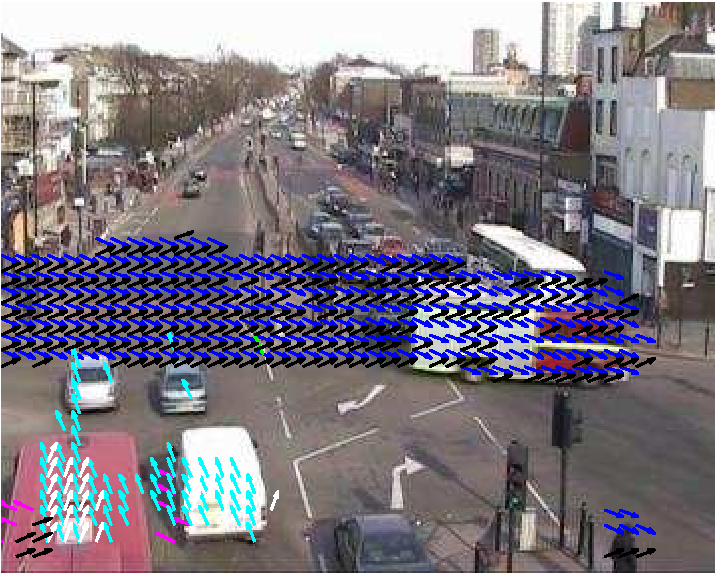
\includegraphics[width=5cm]{figures/qmul/fireengine_414-crop.pdf}
			\centering\scriptsize{Rightward flow in $t+1$ clip}
		\end{minipage}
		\label{fig:fireengine_exsample}
	}
	\caption[Examples of abnormal events]{Three kinds of abnormal events cased by (a) rarely occurring motions, (b) collision activities and (c) impossible state transition according to the traffic rule-}
\end{figure}

\paragraph*{Rare motions.} The first case is the occurrence of unexpected motions. Such motions do not belong to any typical activities. For example as shown in Fig.~\ref{fig:ambulance_exsample}, an ambulance is driving in a forbidden direction in the lane. To detect such abnormal events, we define a word set $x'_t$ in size $N'_t$ as the gathering of motions that do not have any activity label in clip $t$. If $N'_t>Th_{word}$, it is confident that some abnormal motions are existing during this clip.  

\paragraph*{Conflicting Activities.} Second, some activities rarely occurred together with some others during a clip, i.e. in specific traffic state, some specific activities rarely occurred. 
For example, in the state of rightward flow, there should not be any vehicle driving leftward. Fig.~\ref{fig:police_exsample} shows an example of counterflow caused by a police car.
To detect such abnormal events, we use GP regression to model the temporal relationship among different typical activities during a clip. 
As we have discussed in Sec.~\ref{framework:representation}, the feature vector of clip $t$ is denoted as $\mathbf{c}_t=\{p_{t1},\cdots,p_{tK}\}$. The value of $p_{ti}$ has underlying relationship with the others. 
In other words, each value of $\mathbf{c}_t$ can be estimated according to the others in the same clip. Therefore, for each element $p_{ti}$ a GP regression model is constructed. We denote $\mathbf{c}_t^{-p_{ti}}=\{p_{t1},\cdots,p_{tK}\}$ as the input $(K-1)$ dimension features vector and $p_{ti}$ is the corresponding output value,  where $\mathbf{c}_t^{-p_{ti}}$ means that $p_{ti}$ is excluded. Based on the Eq.~\eqref{eq:gpr_prediction}, we make a probabilistic prediction about the output value $p_{ti}$. If the observed value $p_{ti}$ is larger than $\mu+1.96\sigma$, this activity will be vied as conflicting with the others in this clip. $\mu$ is the predicted mean value, $\sigma^2$ is its variance and $(\mu-1.96\sigma,\mu+1.96\sigma)$ is the $95\%$ confidence interval. 
Notice that $p_{ti}$ less than $\mu-1.96\sigma$ is not viewed as conflict, because in practice an activity causes conflict when its intensity is strong enough.
Fig.~\ref{fig:police_exsample} shows an example of identifying the conflicting activities caused by the police car . Each activity is modeled by one GP regression model. Therefore, totally $K$ GP regression models are necessary.

\paragraph*{Illegal State Transition.} Finally, a state is followed by another which is forbidden according to the specific traffic rule. Fig.~\ref{fig:fireengine_exsample} shows an example of an illegal state transition caused by an abnormal event of fire engine interrupting the current vertical traffic flow and driving rightward. The scene is in vertical flow in $t-1$ clip and interrupted by fire engine in $t$ clip. During $t+1$ clip the fire engine is driving cross the scene. Therefore, the $t+1$ clip would be naturally classified as rightward flow with high probability by GP classifier and the result can be modified by Eq.~\eqref{eq:gphmm}. However, no matter based on our human understanding or the clip's features, this recognition is correct. According to the learned state transition rule as shown in Fig.~\ref{qmul_state}, a rightward flow only follows after the leftward flow. Hence, such case should be determined as an abnormal event. We define a logical judgment to identify such abnormal events. If $p(y_t=s_i|y_{t-1}=s_j)= m(s_i,s_j)<Th_{word}$, it will be identified as an illegal state transition, i.e., some abnormal events occur.  

\subsection*{Abnormal Events Localization}
Users are always interesting in the location of of ongoing abnormal events. As discussed in Sec.~\ref{framework:low-level}, each of visual words contains the position information of its cell in the camera scene. Therefore, all visual words belonging to detected abnormal events can be localized. 

We have discussed three kinds of abnormal events and the methods to detect them, respectively. Identifying the abnormal events caused by rare motions and illegal state transition is logic based, which is easy to realize and convenient to apply. 
Different from the methods in \cite{hospedales2011identifying, hospedales2009markov}, Hospedales used LDA model to estimate the likelihood by iterative sweeps of the Gibbs sampler and detected abnormal events which has low posterior. It's really computation and time consuming. 
For the abnormal events caused by conflicting activities, we used GP regression to model the temporal relationship among activities during a clip. It provides a probabilistic analysis of each activity without complex computation.
